\documentclass[colorback,accentcolor=tud1c,11pt]{tudreport}
\usepackage[english]{babel}
\usepackage[utf8x]{inputenc}
%\usepackage[T1]{fontenc}

\usepackage{booktabs}
%\usepackage{multirow}
%\usepackage{longtable}
\usepackage{listings}
\usepackage{graphicx}
\usepackage{subfigure} 	
\usepackage{float}
\usepackage{amsmath}
\usepackage{rotating}
\usepackage{multirow}
\usepackage{colortbl}

\newcommand\todo[1]{\textcolor{red}{#1}}
\newcommand\code[1]{\texttt{#1}}
%\usepackage{floatflt}

\graphicspath{{./img/}}

%\newlength{\longtablewidth}
%\setlength{\longtablewidth}{0.675\linewidth}

\title{Mini-task report: SDC with simulated annealing}
\subtitle{Ludwig Meysel, Mitja Stachowiak}

\begin{document}
  \maketitle

  \chapter{Introduction}
  The task was to implement a simulated annealing approach (SA) for SDC (\underline{s}ystem of \underline{d}ifference \underline{c}onstraints). LPsolve is used to get a schedule for a given set of constraints. The SA-algorithm mutates the order of the constraints to reduce the number of clock cycles of the schedule.
  
  
  
  \chapter{Resources}
  The constraints consist of data flow - and resource constraints. The data flow constraints determine, that no operation must start, before all predecessors have obtained a result. The resource constraints prevent, that the same resource is used twice at the same time.\\
  Each hardware has a certain amount of resources and resource types. There is a fixed list of operations given in the framework:\\
  \begin{tabular}{ c | r | r }
  	Operation name (ar) & delay & weight \\
  	\hline
  	MEM   &  2 & 9.0 \\
  	ADD   &  1 & 1.0 \\
  	SUB   &  1 & 1.4 \\
  	MUL   &  4 & 2.3 \\
  	DIV   & 18 & 4.3 \\
  	SH    &  1 & 2.0 \\
  	AND   &  1 & 2.0 \\
  	OR    &  1 & 2.0 \\
  	CMP   &  1 & 2.1 \\
  	OTHER &  1 & 1.0 \\
  	SLACK &  1 & 0.0 \\
  \end{tabular}\\
  Each resource type can support multiple operations. For this project, the resource(types) are assumed to be overlap-free:
  $$\neg \exists R_1, R_2 \in Resources; Op_1, Op_2 \in Operations : Op_1 \in R_1 \land Op_1 \in R_2 \land Op_2 \in R_1 \land Op_2 \notin R_2$$
  Each resource can handle one operation within a certain time (delay). Multiple resources of the same type may exist.
  



  \chapter{Simulated Annealing}
  The principal structure of any simulated annealing looks like this:\\
  \fbox{\parbox{0.9\linewidth}{
  S = RandomConfiguration();\\
  T = InitialTemperature();\\
  while (ExitCriterion()==false) \{\\
  \phantom{}~~while (InnerLoopCriterion() == false) \{\\
  \phantom{}~~~~S\textsubscript{new} = Generate(S);\\
  \phantom{}~~~~$\Delta$ C = Cost(S\textsubscript{new})-Cost(S);\\
  \phantom{}~~~~r = random(0,1);\\
  \phantom{}~~~~if (r < $e^{- \Delta C/T}$) S = S\textsubscript{new}\\
  \phantom{}~~\}\\
  \phantom{}~~T = updateTemperature();\\
  \}
  }}\\ \\
  The implementation is located in scheduler/SASDC.java:schedule. The parameters are:
  \begin{itemize}
  	\item \emph{Random Configuration} ...
  	\item \emph{Initial Temperature} is determined by applying n(nodes) random changes and saving the costs of each change. T is then $20 * standardDeviation(costs)$.
  	\item \emph{Exit Criterion} is the condition, when the simulated annealing should stop. For each temperature, the number of applied changes and the number of accepted changes is counted. When less then 12\% of the changes are accepted, the algorithm stops.
  	\item \emph{Update Temperature} decreases T by a factor tu, which depends on the acceptance ratio as well:
  	\begin{tabular}{ c | c }
  		acceptance ratio (ar) & temperature factor (tu) \\
  		\hline
  		> 96\% & 0.5 \\
  		96 .. 80\% & 0.9 \\
  		80 .. 15\% & 0.95 \\
  		< 15\% & 0.8 \\
  	\end{tabular}
    \item \emph{Inner Loop Criterion} determines, how many changes are tested for the same temperature. Each change usually moves one node in the ordering of constraint-equations. The larger the number of nodes becomes, the more often each node should be moved, so the number of iterations should depend on the node count. Further more, there is a quality factor $\in [1 .. 10]$ for the algorithm, which can be passed via the third program argument. The formula $n_{inner} = \left\lceil quality * n_{nodes}^{4/3} \right\rceil$ is known to yield a result, thats quality belongs to the given quality.
  \end{itemize}


  \chapter{Details on implementation}

The SDC scheduler with simulated annealing is implemented in the \code{SASDC}-class. The constructor takes the resource constraints and the scheduling quality as parameters. The quality is forwarded to the inner-loop-criterion, which is explained in chapter 3.\par
The actual implementation of the SA algorithm is straight forward, therefore the real point of interest is how the configuration for a schedule is created and how it can be modified with having the option to revert the modification. This is done with a helper class \code{SDCNodeList} (for the sake of simplicity furthermore just called "node list").\par
The node list basically takes the the graph to schedule as constructor parameter. Then it initializes a corresponding \code{Node}-array with a length equals to the number of nodes in the graph. The original \code{Node}-class (from the high-level-framework) has got a new parameter \code{depth}, which is the hierarchical depth of each node (i.e. root-nodes have depth=0, their predecessors have depth=1 and so on). The \code{Node}-array will then be filled ordered by the corresponding depths. This leads to the initial node list which then can be modified in order to optimize the results.\par
To get better results, the list must be reordered somehow, but it must not do "wild swapping" of nodes - the reordering is restricted by the data flow dependencies. To clear this up a bit, figure~\ref{fig:lecturegraph} shows the example graph from the lecture.
\begin{figure}
	\centering
	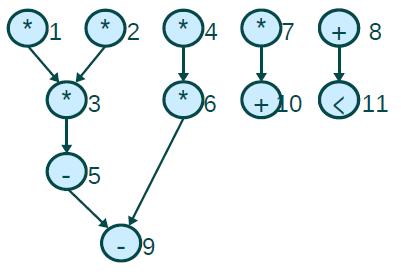
\includegraphics{lecturegraph.png}
	\caption{Example Graph (\cite{Hochberger2017}, Chapter 3, Slide 97)}
	\label{fig:lecturegraph}
\end{figure}

The initial order of the node list (due to the hierarchical depth) could be \#1, \#2, \#4, \#7, \#8, \#3, \#6, \#10, \#11, \#5, \#9. Node \#3 e.g. is a data flow dependency of \#1, \#2, \#5 and \#9. Exactly these dependencies must be considered when \#3 is moved in the list. To be more precise, each predecessor of \#3 must always be left of \#3 and each successor must always be to the right. This restricts the degree of flexibility when modifying the list.\\
To make modification easy, the \code{SDCNodeList} provides two methods \code{shoveRight} and \code{shoveLeft}, which do the following:

%
% BITTE PSEUDOCODE DRAUS MACHEN (KANNS BEI MIR NICHT TESTEN)
%
shoveRight(i0: int):
	// nodes is a class-member
	shoveCount: int
	for(int i := i0+1; i < nodes.length; i++)
		// find first non-flow-dependend-node
		if (nodes[i] isNoSuccessorOf nodes[i0])
			shoveCount = i - i0;
			break;

	// move items  [i0 ... i0 + shoveCount] one array i0 to the right
	// set original item from list[i0] = list[i0 + shoveCount]

This is a generic example and works in almost the same manner for shoveLeft. Basically the shove-functions find the first non-dependend predecessor/successor node beginning searching at \code{i0}. The initial ordering in the example before ended with the nodes \#11, \#5, \#9. When shoving \#9 to the left, the first node which would be checked to be predecessor is \#5. Next iteration, \#11 fulfils the \textit{isNoPredecessor}-criterion, therefore the \code{shoveCount} would be set to 2 and the loop cancels. Now the elements would be reordered to \#5, \#9, \#11.\par
By storing the \code{i0} and \code{shoveCount}, the operation can easily be reverted if the change is not accepted the SA algorithm.
	



  \chapter{Evaluation}
  \vspace{100pt}
  \begin{tabular}{ c | r | r | r | r | r | r | r }
    File &
    \begin{rotate}{60} Number of Nodes \end{rotate} \hspace{3pt} &
    \begin{rotate}{60} cost fkt of ASAP \end{rotate} \hspace{10pt} &
    \begin{rotate}{60} cost fkt of ALAP \end{rotate} \hspace{10pt} &
    \begin{rotate}{60} cost fkt of SA/SDC \end{rotate} \hspace{10pt} &
    \begin{rotate}{60} Quality factor of SA \end{rotate} \hspace{3pt} &
    \begin{rotate}{60} Number of Iterations \end{rotate} \hspace{12pt} &
    \begin{rotate}{60} Runtime / s \end{rotate} \hspace{12pt} \\
   \hline
   \multirow{3}{*}{ADPCMn-decode-271-381} & \multirow{3}{*}{27} & \multirow{3}{*}{64.8} & \multirow{3}{*}{56.0} & 31.9 & 1 & 20494 & 29.39 \\
    &  &  &  & 30.5 & 5 & 82216 & 113.38 \\
    &  &  &  & 30.5 & 10 & 144181 & 185.55 \\ \arrayrulecolor{gray}\hline
   \multirow{3}{*}{ADPCMn-decode-425-472} & \multirow{3}{*}{12} & \multirow{3}{*}{23.8} & \multirow{3}{*}{23.8} & 34.2 & 1 & 85 & 0.11 \\
    &  &  &  & 21.8 & 5 & 7591 & 6.37 \\
    &  &  &  & 21.8 & 10 & 11001 & 9.13 \\ \arrayrulecolor{gray}\hline
   \multirow{3}{*}{ADPCMn-decode-524-553} & \multirow{3}{*}{7} & \multirow{3}{*}{25.4} & \multirow{3}{*}{26.4} & 25.4 & 1 & 15 & 0.02 \\
    &  &  &  & 25.4 & 5 & 68 & 0.07 \\
    &  &  &  & 25.4 & 10 & 135 & 0.13 \\ \arrayrulecolor{gray}\hline
   \multirow{3}{*}{ADPCMn-decode-559-599} & \multirow{3}{*}{9} & \multirow{3}{*}{26.1} & \multirow{3}{*}{27.2} & 28.2 & 1 & 20 & 0.03 \\
    &  &  &  & 25.1 & 5 & 4137 & 3.26 \\
    &  &  &  & 28.2 & 10 & 377 & 0.35 \\ \arrayrulecolor{gray}\hline
   \multirow{3}{*}{ADPCMn-decode-631-729} & \multirow{3}{*}{23} & \multirow{3}{*}{44.8} & \multirow{3}{*}{40.0} & 33.3 & 1 & 5017 & 5.81 \\
    &  &  &  & 24.3 & 5 & 13121 & 14.65 \\
    &  &  &  & 22.9 & 10 & 108076 & 120.56 \\ \arrayrulecolor{gray}\hline
   \multirow{3}{*}{ADPCMn-decode-771-791} & \multirow{3}{*}{5} & \multirow{3}{*}{13.5} & \multirow{3}{*}{13.5} & 22.5 & 1 & 10 & 0.01 \\
    &  &  &  & 22.5 & 5 & 44 & 0.04 \\
    &  &  &  & 22.5 & 10 & 87 & 0.08 \\ \arrayrulecolor{gray}\hline
   \multirow{3}{*}{ADPCMn-decode-803-832} & \multirow{3}{*}{8} & \multirow{3}{*}{18.8} & \multirow{3}{*}{18.8} & 20.2 & 1 & 17 & 0.02 \\
    &  &  &  & 20.2 & 5 & 81 & 0.08 \\
    &  &  &  & 20.2 & 10 & 161 & 0.16 \\ \arrayrulecolor{gray}\hline
   \multirow{3}{*}{AESrkgcyclic} & \multirow{3}{*}{24} & \multirow{3}{*}{24.4} & \multirow{3}{*}{23.4} & 37.4 & 1 & 421 & 0.61 \\
    &  &  &  & 32.4 & 5 & 13881 & 18.84 \\
    &  &  &  & 30.4 & 10 & 28414 & 38.14 \\ \arrayrulecolor{gray}\hline
   \multirow{3}{*}{BLAKE256Digest-processBlock-160-230} & \multirow{3}{*}{21} & \multirow{3}{*}{57.4} & \multirow{3}{*}{58.4} & 32.4 & 1 & 10905 & 12.11 \\
    &  &  &  & 22.4 & 5 & 58291 & 64.11 \\
    &  &  &  & 31.4 & 10 & 175161 & 194.06 \\ \arrayrulecolor{gray}\hline
   \multirow{2}{*}{BLAKE256Digest-processBlock-189-1577} & \multirow{2}{*}{308} & \multirow{2}{*}{414.9} & \multirow{2}{*}{128.7} & 110.9 & 1 & 6244 & 241.63 \\
    &  &  &  & 97.9 & 5 & 31204 & 1236.87 \\ \arrayrulecolor{gray}\hline
   \multirow{3}{*}{ContrastFilter-filter-13-252} & \multirow{3}{*}{47} & \multirow{3}{*}{72.0} & \multirow{3}{*}{67.7} & 50.8 & 1 & 4251 & 9.49 \\
    &  &  &  & 37.7 & 5 & 24622 & 54.00 \\
    &  &  &  & 33.2 & 10 & 101821 & 218.61 \\ \arrayrulecolor{gray}\hline
   \multirow{1}{*}{ECOH256Digest-AES2RoundsAll-2-666} & \multirow{1}{*}{179} & \multirow{1}{*}{262.3} & \multirow{1}{*}{174.4} & 58.1 & 1 & 175567 & 2733.60 \\
  \end{tabular}\\ \\
  The table above compares the results of simple ASAP / ALAP-Schedules with the results of the implemented simulated annealing algorithm.
 


 
 \chapter{Conclusion}
 

%  \bibliographystyle{plain}
%  \bibliography{references}
\end{document}

